% To je predloga za poročilo projekta pripredmetu Osnove verjetnosti in
% statistike.
% Originalen avtor predloge je Blaž Zupan.
% Za potrebe OVS je prilagodil Robert Cvitkovič
% To predlogo lahko spremeniš v PDF dokument s pomočjo programa
% pdflatex, ki je del standardne instalacije LaTeX programov.

\documentclass[a4paper,11pt]{article}
\usepackage[utf8]{inputenc}
\usepackage{amsmath, amssymb, amsthm, amsfonts, mathtools}
\usepackage{a4wide}
\usepackage[slovene]{babel}
\usepackage{graphicx}
\usepackage{url}
\usepackage{float}
\usepackage[pdftex,pdfpagelabels,bookmarks,hyperindex,hyperfigures]{hyperref}
% \usepackage{hyperref}
\hypersetup{
pdffitwindow=true,              % window fit to page when opened
pdftitle={Seminarska pri predmetu VIS},       % title
pdfauthor={Matej Kalc},                % author
pdfnewwindow=true,              % links in new window
colorlinks=true,                % false: boxed links; true: colored links
linkcolor=blue,                 % color of internal links
citecolor=blue,                 % color of links to bibliography
filecolor=blue,                 % color of file links
urlcolor=cyan                   % color of external links
}

% \usepackage{tikz}
% \usepackage{pgflibraryshapes}

\usepackage[footnotesize,labelfont=bf,labelsep=period]{caption}
\usepackage{enumerate}

\newcommand{\doi}[1]{\href{http://dx.doi.org/#1}{\texttt{doi:#1}}}
\newcommand{\arxiv}[1]{\href{http://arxiv.org/abs/#1}{\texttt{arXiv:#1}}}
\graphicspath{ {./Slike/} }


\title{Potek širjenja do viška Covid-19 v Evropi}
\author{Matej Kalc} % (63180368)}
\date{\today}

\begin{document}

\maketitle

\section{Uvod}
\subsection{Motivacija}

% V tem razdelku, 
% ki naj bo kratek in naj obsega en odstavek z do 150 besed, 
% na kratko opišeš, kaj je bil cilj naloge.

\emph{“Koronavirus je hujši kot vojna, kjer je sovražnik še vedno človek, s katerim se še
vedno lahko ukvarjamo, medtem ko je kakršenkoli dogovor s smrtonosnim virusom,
ki ogroža naše preživetje, nemogoč. (...)".} \\ \\
Tako je izjavil G. Zuccarini. Lahko bi izjavili, da je Koronavirus tretja svetovna vojna, kjer se neviden sovražnik skriva med ljudmi. Ogroža ljudem življenje, nekaterim pa ga tudi odvzame. Ljudje lahko premagamo nevidnega sovražnika, le če primerno in provočasno ukrepamo s pravim orožjem, kot so samozavest in ukrep človeka. V taki bitki tudi študiji in analize podatkov so dobro orožje proti virusu, saj izvemo nekaj novega o našem sovražniku. Mogoče eden izmed teh nam bom dal možnost odkritja cepiva zdravilo proti virusu, toda dokler tega ne ugotovimo ostaja edina možnost uporaba mask, razkužil in podobno. Zanima me kako so ljudje odzvali na epidemijo. Zanima me katere države so bile najboljše in katere najslabše organizirane za preprečevanje okužbe. Ker je epidemija še v teku, bom kot vzorec izbral države Evropske Unije, ker se je v teh epidemija sprožila približno sočasno. 


\subsection{Cilji}
Trdimo lahko, da so vse države v Evropski uniji preživele prvi val Koronavirus pred 19.julijem 2020. V seminarski bom analiziral kako se je virus širil po državah EVropske unije. Predvsem bom analiziral interval od začetka širjenja do vrhunca prvega vala virusa v vsaki evropski državi, ker je ta interval najzanimivejši, saj so v tem intervalu evropske države prvič pod vplivom virusa. Zanima nas tudi kako je vsaka država Evropske unije začela testrati, tako da bo zmanjšala bodoče okužbe. \\
Cilj študija je analiza:
\begin{itemize}
\item{Vpliva media starosti populacije EU države na smrtonosnost virusa, }
\item{Vpliva števila dni do viška dnevnih okuženih primerov na delež okuženih do viška in }
\item{Vpliva velikosti populacije na število opravljenih testov. }
\end{itemize}
Testiral bom korelacijo med spremenljivkami. Izračunal bom intervale zaupanja, saj podatki niso realni, ker v teh niso vsebovani asimptomatici (KAKO SE REČE?).


\subsection{Raziskave o virusu}
Veliko je spletnih strani, ki analizirajo in grafično prikazujejo podatke Covid-19. Naštel bom eno, ki me je motivirala za seminarsko. \\
Inštitut za zdravstvene meritve in vrednotenje IHME nudi spletno stran o Koronavirus, kjer so grafično prikazani podatki o okuženih, mrtvih, testih, socialna distanca ipd, ampak najzanimivejše so projekcije v času, ki stran nudi. IHME-ove projekcije COVID-19 so bile razvite kot odziv na zahteve Medicinske šole Univerze v Washingtonu in drugih ameriških bolnišničnih sistemov in vladnih držav, ki si prizadevajo za določitev, kdaj bo COVID-19 premagal njihovo sposobnost oskrbe bolnikov. Napovedi kažejo povpraševanje po bolnišničnih storitvah, dnevne in kumulativne smrti zaradi COVID-19, stopnje okužbe in testiranja ter vpliv socialne distanciranja, ki ga organizira država in država (za izbrane lokacije).

\subsection{Poglavja}
\begin{enumerate}
\item{Uvod}
\item{Opis virusa in njegovo širjenje}
\item{Podatki}
\item{Izračuni in rezultati}
\item{Zaključki}
\item{Literatura}
\end{enumerate}

\section{Opis virusa in njegovo širjenje}
COVID-19 je nalezljiva bolezen, ki jo povzroča virus SARS-CoV-2. Dihalni virus se širi preko kašlja in kihanja. Prvi okuženec Covid-19 je bil zaznan na Kitajskem novembra 2019. Najprej se je dihaln virus širil na Kitajskem, Hubei in Wuhan. Na začetku leta 2020 se je začelo širjenje virusa po celem svetu. 11. marca 2020 je Svetovna zdravstvena organizacija WHO proglasila pandemijo. Iz statističnih podatkov je razvidno, da do vključno 19. julija 2020 je bilo okuženih več kot 14.2 milijonov ljudi v 188 državah, od katerih 600 tisoč je mrtvih in 8.02 milijonov je ozdravelih. Trdimo lahko, da je ta virus leta 2020 močno vplival na države po celem svetu.
\section{Podatki}
Podatki so bili izbrani iz spleta. Podatke, ki bom rabil za statistični študij, so:
\begin{enumerate}
\item{Seznam Evropskih držav}
\item{Povprečna starost populacije vsake Evropske države}
\item{Število prebivalcev vsake Evropske države}
\item{Dnevno število mrtvih v vsaki Evropski državi}
\item{Dnevno število okuženih v vsaki Evropski državi
\item{Datum vrhunca števila okuženih prvega vala v vsaki Evropski državi}
\item{Datum vrhunca števila mrtvih prvega vala v vsaki Evropski državi}
\item{Dnevno število opravljemoh testov v vsaki Evropski državi}
\item{Število mrtvih do vrhunca prvega vala v vsaki Evropski državi}
\item{Število okuženih do vrhunca prvega vala v vsaki Evropski državi}
\end{enumerate}

Število mrtvih do vrhunca prvega vala v vsaki Evropski državi (9) je seštevek dnevno število mrtvih v vsaki Evropski državi(4) od datuma prvega mrtvega zaradi virusa do datum vrhunca števila mrtvih prvega vala v vsaki Evropski državi(7).
Število okuženih do vrhunca prvega vala v vsaki Evropski državi (10) je seštevek dnevno število okuženih v vsaki Evropski državi(5) od datuma prvega mrtvega zaradi virusa do datum vrhunca števila okuženih prvega vala v vsaki Evropski državi(6).

\section{Izračuni in rezultati}
Podatki iz prvega vala nam povejo koliko je bila država pripravljena na tako epidemijo.

\subsection{Vpliv mediane starosti EU države na fatalnost virusa Covid-19}
Zanima me kako se je širjenje razlikovalo med Evropskimi državami in sicer prvo moje vprašanje je: Je fatalnost virusa pod vplivom mediane starosti populacije?

Najprej definiramo fatalnost.
\begin{center}
\[\textbf{fatalnost} = \frac{\text{število mrtvih}}{\text{število okuženih}}\]
\end{center} 
Fatalnost je neka vrednost med 0 in 1, torej nek procent. Naj bo fatalnost prve polovice prvega vala razmerje med številom mrtvih prve polovice prvega vala in številom okuženih prvega vala. \\
Za analizo vzamemo spremenljivki F in S, kjer F predstavlja fatalnost in S mediano starosti države. Spremenljivki F in S vsake države evropske unije sta prikazani v spodnjem grafu.
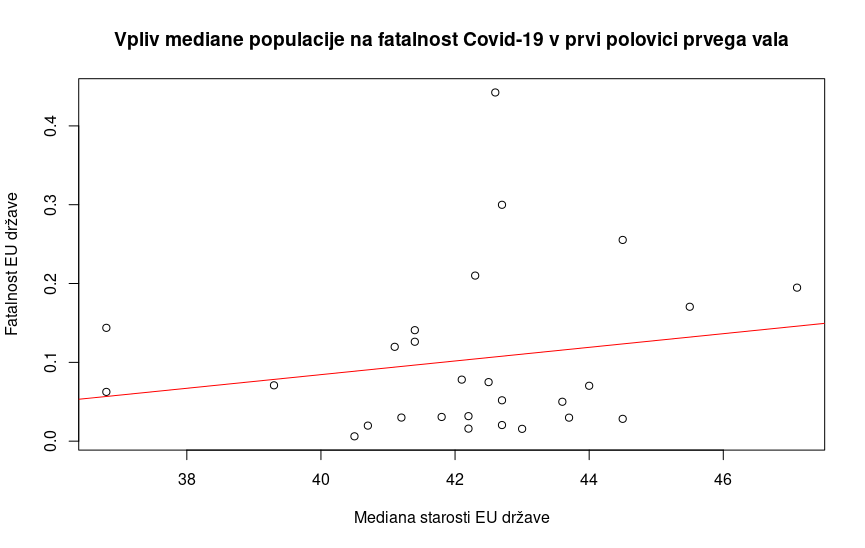
\includegraphics[scale=0.7]{Vpliv_mediane_populacije_na_fatalnost_Covid-19_v_prvi_polovici_vala}

\subsection{Vpliv števila dni do viška dnevnih okuženih primerov na delež okuženih do viška}
\subsection{Vpliv velikosti populacije na število opravljenih testov}


\section{Zaključki}
\section{Literatura}
https://en.wikipedia.org/wiki/List_of_countries_by_median_age \\
https://en.wikipedia.org/wiki/Europe \\
https://en.wikipedia.org/wiki/List_of_European_countries_by_population \\
https://covid19.healthdata.org/ \\
https://covid19.who.int/info \\
https://github.com/KalcMatej99/Seminarska-VS-Covid-19 \\


\end{document}
